\documentclass{article}
\usepackage[fleqn]{amsmath}
\usepackage[pointsonleft,nototals,
    forcolorpaper,useforms,
% choose to compile with exactly one of the next 4 options
%-------------------
    nosolutions,    % compile with no solutions to get the exam document
%   answerkey,      % get answer key
%   vspacewithsolns,% put solutions at end of document
%   solutionsonly,  % compile with vspacewithsolns several times, then compile with solutionsonly
%-------------------
%   coverpage,coverpagesumry=bypages
    showgrayletters]{eqexam}
\usepackage{graphicx}

\forceNoColor
\vspacewithkeyOn

\university
{%
      NORTHWEST FLORIDA STATE COLLEGE\\
         Department of Mathematics
}
\email{storyd@nwfsc.edu}

\examSIDLabel{Class: MAC 1105, \vA{12:30 pm, L-134}\vB{12:30 am, L-105}}
\coverpageSubjectFmt{\bfseries\LARGE}
\coverpageTitleFmt{\bfseries\LARGE}
\examNum{3}\numVersions{2}\forVersion{a}
\subject[MAC1105]{College Algebra}
\longTitleText
    {Test~\nExam}
    {Test~\nExam}
\endlongTitleText
\shortTitleText
    {T\nExam}
    {T\nExam}
\endshortTitleText
\altTitle{\vA{12:30 pm, L-134}\vB{12:30 pm, L-105}}
\title[\sExam]{\Exam}
\author{Dr.\ D. P. Story}
\date{\thisterm, \the\year}
\duedate{04/05/11}
\keywords{MAC 1105, Exam \nExam, {\thisterm} semester, \theduedate, at NWFSC}
\renewcommand{\fillInFormatDefault}{}
\DoNotFitItIn
\eqpartsitemsep{3pt}
\solAtEndFormatting{\eqequesitemsep{3pt}}


\everymath{\displaystyle}
%\renameSolnAfterTo{}
%\resetSolnAfterToDefault


\eqCommentsColor{gray}
\eqCommentsColorBody{gray}
\newcommand{\cs}[1]{\texttt{\char`\\#1}}
\def\qt#1{&&\qquad\text{#1}}


\encloseProblemsWith{theseproblems}

\begin{document}

\maketitle


\begin{exam}{Test\nExam}

\ifsolutionsonly\NoPoints
\begin{instructions}[Solutions:]
The solutions to the test.
\end{instructions}
\else
\begin{instructions}[Instructions:]
This exam has {\nQuesInExam} questions distributed over {\nPagesOnExam} pages.
Solve each of the problem and box in your final $\boxed{\text{answer}}$, where applicable.
\end{instructions}
\fi

\begin{theseproblems}

\renameSolnAfterTo{}

\begin{problem*}[2ea]\label{shortAns}
Answer each of the following, none of the problems shown below requires any
calculations. Respond to True/False questions with \texttt{T} (for True) or \texttt{F} (for
False).
\begin{parts}
    \item When viewing the graph of a function, we may use the
    \fillin[u]{1.5in}{Horizontal Line} Test to determine if it is a
    one-to-one function.
\begin{solution}[]\ifvspacewithsolns
When viewing the graph of a function, we may use the
\fillin[u]{1.5in}{Horizontal Line} Test to determine if it is a
one-to-one function.\fi
\end{solution}

    \item \TF{F} (\texttt{T} or \texttt{F}) The graph of the function $ f(x) =
    2-4x-3x^2$ is a parabola that opens up.
\begin{solution}[]\ifvspacewithsolns
\TF{F} (\texttt{T} or \texttt{F}) The graph of the function $ f(x) =
2-4x-3x^2$ is a parabola that opens up.\fi
\end{solution}

    \item \TF{F} (\texttt{T} or \texttt{F}) For a quadratic function of the form
    $f(x)=ax^2+bx+c$, if $a>0$, then the function has a \emph{maximum
    value}.
\begin{solution}[]\ifvspacewithsolns
\TF{F} (\texttt{T} or \texttt{F}) For a quadratic function of the form
    $f(x)=ax^2+bx+c$, if $a>0$, then the function has a \emph{maximum
    value}.\fi
\end{solution}

\pushProblem

\begin{eqComments}[Comments:]
Questions like the three above (fill-in and True/False) often have no
solution; hence, normally, the \texttt{solution} environment is not used. When
using the \texttt{vspacewithsolns} or the \texttt{solutionsonly} options
you would like the ``answers'' to appear on the solutions pages. To
rectify this, we simply copy and past the item into a solutions
environment, like so, in the case of the last question above.
\begin{verbatim}
\begin{solution}[]\ifvspacewithsolns
\TF{F} (\texttt{T} or \texttt{F}) For a quadratic function of the form
    $f(x)=ax^2+bx+c$, if $a>0$, then the function has a \emph{maximum
    value}.\fi
\end{solution}
\end{verbatim}
The optional argument is empty (important). We don't want the student or instructor to
see this solution when the document is compiled using the \texttt{answerkey}
option, so we wrap this solution in a conditional
\verb~\ifvspacewithsolns...\fi~ This switch will be true if either the
options \texttt{vspacewithsolns} or \texttt{solutionsonly} options are
taken
\end{eqComments}

\popProblem

    \item\label{whichRatFunc} Which rational function below has a horizontal asymptote of
    $y=-2$, and has vertical asymptotes of $x=1$ (odd) and $ x=2 $ (even)?
    \begin{answers}{3}\rowsep{6pt}
    \bChoices[label=whichRat]
        \Ans0 $ y = \frac{(x+2) (1-2x)}{(1-x)(x-2)^2} $\eAns
        \Ans0 $ y = \frac{(x+2)^2 (2x-1)}{(x-1)(x-2)^2} $\eAns
        \Ans1 $ y = \frac{(x+2)^2 (1-2x)}{(x-1)(x-2)^2} $\eAns
        \Ans0 $ y = \frac{(x+2)^2 (2x-1)}{(x-1)^2(x-2)} $\eAns
        \Ans0 $ y = \frac{(x+2) (1-2x)^2}{(x-1)^2(x-2)} $\eAns
        \Ans0 none of these\eAns
    \eChoices
    \end{answers}
\begin{solution}[]\ifvspacewithsolns
We can access the ``answers'' to a multiple choice question in several
ways:
\begin{itemize}
\item The correct alternative is part~\useSavedAlts{whichRat},
\useSavedAns{whichRat}.
\begin{verbatim}
The correct alternative is part~\useSavedAlts{whichRat},
\useSavedAns{whichRat}.
\end{verbatim}
The command \verb!\useSavedAlts{whichRat}! expands to the letter alternative of the
correct response, \useSavedAlts{whichRat}, in this case. Similarly,
\verb!\useSavedAns{whichRat}! expands to the correct answer, here, the
correct answer is \useSavedAns{whichRat}.

\item The correct answer is \useSavedAltsAns{whichRat}.
\begin{verbatim}
The correct answer is \useSavedAltsAns{whichRat}.
\end{verbatim}
The command \verb!\useSavedAltsAns{whichRat}! expands to the correct
letter followed by the correct answer.
\item You can  now copy and paste the \texttt{answers} (or \texttt{manswers})
      environment into the \texttt{solutions} environment, like so.

\item[] Which rational function below has a horizontal asymptote of
    $y=-2$, and has vertical asymptotes of $x=1$ (odd) and $ x=2 $ (even)?
    \begin{answers}{3}\rowsep{6pt}
    \bChoices[label=whichRat]
        \Ans0 $ y = \frac{(x+2) (1-2x)}{(1-x)(x-2)^2} $\eAns
        \Ans0 $ y = \frac{(x+2)^2 (2x-1)}{(x-1)(x-2)^2} $\eAns
        \Ans1 $ y = \frac{(x+2)^2 (1-2x)}{(x-1)(x-2)^2} $\eAns
        \Ans0 $ y = \frac{(x+2)^2 (2x-1)}{(x-1)^2(x-2)} $\eAns
        \Ans0 $ y = \frac{(x+2) (1-2x)^2}{(x-1)^2(x-2)} $\eAns
        \Ans0 none of these\eAns
    \eChoices
    \end{answers}
\end{itemize}\fi
\end{solution}

\pushProblem
\begin{eqComments}[Comments:]
Multiple choice and multiple selection questions were an especially
difficult problem to solve; the \texttt{answers} and \texttt{manswers}
environments are undefined outside of an \texttt{exam} environment so one
cannot simply copy and paste the choices into the \texttt{solution} environment.

To resolve this issue, I added a key-value pair to the \cs{bChoices} command,
the key is \texttt{label}. The source code for the above question reads
\verb!\bChoices[label=whichRat]! The value of the label key is used to
build a series of macros that record the labels and text for the choices
that are marked correct by \cs{Ans1}. The information gathered by these
macros are accessible through \cs{useSavedAlts}, \cs{useSavedAns},
\cs{useSavedAltsAns}, and \cs{useSavedNumAns}, as described in the \textsf{eqexam}
manual. See the solutions pages to see the answers to these multiple
choice questions and details on the use of these commands.
\end{eqComments}
\popProblem

    \item How many times can a quadratic equation cross the $x$-axis?
    Check as many of the alternatives that are possibly correct for a
    quadratic function.
    \begin{manswers}{4}
    \bChoices[label=nCrossings]
        \Ans1 0\eAns
        \Ans1 2\eAns
        \Ans1 3\eAns
        \Ans0 4\eAns
        \Ans0 5\eAns
        \Ans0 6\eAns
        \Ans0 infinitely many\eAns
        \Ans0 none of these\eAns
    \eChoices
    \end{manswers}
\begin{solution}[]\ifvspacewithsolns
Here is how these same macros expand for multiple selection problems.
\begin{itemize}
\item The correct alternatives are parts~\useSavedAlts{nCrossings}.
\begin{verbatim}
The correct alternatives are parts~\useSavedAlts{nCrossings}.
\end{verbatim}
\item The correct answers are \useSavedAns{nCrossings}.
\begin{verbatim}
The correct answers are \useSavedAns{nCrossings}.
\end{verbatim}
\item The correct responses are \useSavedAltsAns{nCrossings}.
\begin{verbatim}
The correct responses are \useSavedAltsAns{nCrossings}.
\end{verbatim}
\item[] End each case, the command expands to a comma-delimited list of correct
answers.
\end{itemize}
You can also access the answers individually, for example the second
correct response is part~\useSavedAlts[2]{nCrossings}, the answer for
part~\useSavedAlts[2]{nCrossings} is \useSavedAns[2]{nCrossings}. Or,
we can say, \useSavedAltsAns[2]{nCrossings} to get a combined listing of
the second correct response.
\begin{verbatim}
You can also access the answers individually, for example the second
correct response is part~\useSavedAlts[2]{nCrossings}, the answer for
part~\useSavedAlts[2]{nCrossings} is \useSavedAns[2]{nCrossings}. Or,
we can say, \useSavedAltsAns[2]{nCrossings} to get a combined listing of
the second correct response.
\end{verbatim}
\fi
\end{solution}
\end{parts}
\end{problem*}

\begin{eqComments}[Comments:]
The above question is a multiple selection question. The student must
select all the correct choices. See the solutions pages to see the answers
to these multiple choice questions and details on the use of these
commands.
\end{eqComments}

\begin{problem}[5]
Which rational function below has a horizontal asymptote of
    $y=-2$, and has vertical asymptotes of $x=1$ (odd) and $ x=2 $ (even)?
    \begin{answers}{3}\rowsep{6pt}
    \bChoices[label=whichRat1]
        \Ans0 $ y = \frac{(x+2) (1-2x)}{(1-x)(x-2)^2} $\eAns
        \Ans0 $ y = \frac{(x+2)^2 (2x-1)}{(x-1)(x-2)^2} $\eAns
        \Ans1 $ y = \frac{(x+2)^2 (1-2x)}{(x-1)(x-2)^2} $\eAns
        \Ans0 $ y = \frac{(x+2)^2 (2x-1)}{(x-1)^2(x-2)} $\eAns
        \Ans0 $ y = \frac{(x+2) (1-2x)^2}{(x-1)^2(x-2)} $\eAns
        \Ans0 none of these\eAns
    \eChoices
    \end{answers}
\begin{solution}[]\ifvspacewithsolns
We can access the ``answers'' to a multiple choice question in several
ways:
\begin{itemize}
\item The correct alternative is part~\useSavedAlts{whichRat1},
\useSavedAns{whichRat1}.
\begin{verbatim}
The correct alternative is part~\useSavedAlts{whichRat1},
\useSavedAns{whichRat1}.
\end{verbatim}
The command \verb!\useSavedAlts{whichRat1}! expands to the letter alternative of the
correct response, \useSavedAlts{whichRat1}, in this case. Similarly,
\verb!\useSavedAns{whichRat1}! expands to the correct answer, here, the
correct answer is \useSavedAns{whichRat1}.

\item The correct answer is \useSavedAltsAns{whichRat1}.
\begin{verbatim}
The correct answer is \useSavedAltsAns{whichRat1}.
\end{verbatim}
The command \verb!\useSavedAltsAns{whichRat1}! expands to the correct
letter followed by the correct answer.
\end{itemize}\fi
\end{solution}
\end{problem}

\begin{eqComments}[Comments:]
This is the same question as Problem~\ref{shortAns} (\ref{whichRatFunc}),
but this one is a stand alone question.  The lettering of the label can
change depending on the options you take, so, if you compile this document
without the \texttt{useforms} options, the choices listed in~\ref{shortAns} (\ref{whichRatFunc})
will be numbers, (A), (B),\dots, and the choices of this question will be
letters, (a), (b),\dots. Check the solutions page, the references should
change to reflect the change in options, let's hope.
\end{eqComments}

\resetSolnAfterToDefault

\begin{problem*}[\auto]
Let $f(x) = 4x+3$ and $ g(x) = 2x^2 - 5 $. Compute each of the following,
simplify were appropriate.
\begin{multicols}{2}
\begin{parts}
\item \PTs{2} $ (fg)(-2) = \fillin[boxed,boxsize=LARGE,align=l]{1in}{-15} $

\begin{solution}[.65in]
We have \[ (fg)(-2)=f(-2)g(-2)=(-5)(3)=\boxed{-15}\]
\end{solution}

\item \PTs{2} $\left(\frac{g}{f}\right)(x)= \fillin[boxed,boxsize=LARGE]{\ifNoSolutions{1in}{}}{\frac{2x^2-5}{4x+3}} $

\begin{solution}[\sameVspace]
$ \left(\frac{g}{f}\right)(x)=\frac{g(x)}{f(x)}=\boxed{\frac{2x^2 - 5}{4x+3}}$
\end{solution}

\item \PTs{2} $ (f\circ f )(x)  = \fillin[boxed,boxsize=LARGE]{\ifNoSolutions{1in}{}}{16x+15} $

\begin{solution}[\sameVspace]
Composing, $(f\circ f )(x)=f(f(x))=f(4x+3)=4(4x+3)+3=\boxed{16x+15}$
\end{solution}

\item \PTs{4} $ (f\circ g )(x)  = \fillin[boxed,boxsize=LARGE]{1in}{8x^2-17} $

\begin{solution}[\sameVspace]
Composing, $(f\circ g )(x)=f(g(x))=f(2x^2 - 5)=4(2x^2 -5)+3=\boxed{8x^2-17}$
\end{solution}
\end{parts}
\end{multicols}
\end{problem*}

\begin{eqComments}[Comments:]
Nothing new about the above problem, each has a solution, no special
attention is needed. In some of the answer boxes, \cs{ifNoSolutions} is
used to set the width then \texttt{nosolutions} is in effect, and to et the box to
its natural width otherwise.
\end{eqComments}


\begingroup

\setlength{\columnsep}{30pt}

\begin{multicols}{2}
\begin{problem}[5]
Use the \textbf{vertex formula} to find the $x$-coordinate, $h$, and the
$y$-coordinate, $k$, of the quadratic function $ f(x) = 2x^2 - 8x + 5 $.
\begin{equation*}
    \fillin[boxed,boxsize=LARGE,align=l,boxpretext={h=}]{1in}{2}\quad
    \fillin[boxed,boxsize=LARGE,align=l,boxpretext={k=}]{1in}{-3}
\end{equation*}
\begin{solution}[.5in]
We use the vertex formula, $ h = -b/(2a) = - (-8)/4 = 2 $, and
so $h=f(2) = 8 - 16 + 5 = -3$.
\end{solution}
\end{problem}

\columnbreak

\begin{problem}[] %
\PTs{3}\addtocounter{eqpointvalue}{3} The function $ f(x) = x^2 - x + 1 $ has a
\fillin[u]{.75in}{minimum} (max/min) at $x = \fillin[u]{.5in}{1/2}$.
\begin{solution}[\sameVspace]
We use the vertex formula, $ h = -b/(2a) = - (-1)/2 =
1/2 $. A \textbf{minimum} occurs since the leading coefficient is
positive, which means the parabola opens up, the vertex is a minimum.
\end{solution}
\end{problem}
\end{multicols}

\endgroup

\begin{eqComments}[Comments:]
I include this problem in this file, because it is a construct that
appeared in a test of mine. I wanted to conserve vertical space so I put
to problems into two column format. The problem is the points appear to
the left. So, for the problem on the left, the points appear as usual, for
the problem on the right, the points appear in-line, I had to explicitly
increment the points counter, like so
\verb~\addtocounter{eqpointvalue}{3}~. Some adjustment of the space
between the columns was necessary \verb~\setlength{\columnsep}{30pt}~.
\end{eqComments}

\renameSolnAfterTo{}

\begin{problem}[5]
For a polynomial of degree $12$, according to theory, the maximum number
of zeros is \fillin[u]{.5in}{12}, and the maximum number of turning points
is \fillin[u]{.5in}{11}.
\begin{solution}[]\ifvspacewithsolns
For a polynomial of degree $12$, according to theory, the maximum number
of zeros is \fillin[u]{.5in}{12}, and the maximum number of turning points
is \fillin[u]{.5in}{11}.\fi
\end{solution}
\end{problem}

\begin{eqComments}[Comments:]
A fill-in the blank problem, just copy and paste it into the solution
environment, protected by \verb~\ifvspacewithsolns...\fi~.
\end{eqComments}


\begin{problem}[5]
In the boxes provided, list the laws of the exponents and the laws of
logarithms.
    \begin{equation*}\def\bwidth{2.75in}\def\bheight{1.5in}
        \begin{tabular}{cc}
        \textbf{Laws of the Exponents} & \textbf{Laws of Logarithms}\\
        \multicolumn{1}{p{\bwidth}}{%
        \fillin[boxed,enclosesoln,parbox={[c][\bheight][t]}]{\linewidth}{%
%
        \begin{enumerate}
            \item $a^x a^y = a^{x+y}$
            \item $a^x/a^y = a^{x-y}$
            \item $ (a^x)^y = a^{xy}$
        \end{enumerate}
%
        }}&
        \multicolumn{1}{p{\bwidth}}{%
        \fillin[boxed,enclosesoln,parbox={[c][\bheight][t]}]{\linewidth}{%
%
        \begin{enumerate}
            \item $\log_a(xy) = \log_a(x)+\log_a(y)$
            \item $\log_a(x/y) = \log_a(x)-\log_a(y)$
            \item $\log_a(x^r) = r\log_a(x)$
        \end{enumerate}
%
        }}
        \end{tabular}
    \end{equation*}
\begin{solution}[]\ifvspacewithsolns
Write sentences, in the provided boxes, describing,  in laymen's terms, Type I
    and Type II errors for this test of hypothesis.
    \begin{equation*}\def\bwidth{2.75in}\def\bheight{1.5in}
        \begin{tabular}{cc}
        \textbf{Laws of the Exponents} & \textbf{Laws of Logarithms}\\
        \multicolumn{1}{p{\bwidth}}{%
        \fillin[boxed,enclosesoln,parbox={[c][\bheight][t]}]{\linewidth}{%
%
        \begin{enumerate}
            \item $a^x a^y = a^{x+y}$
            \item $a^x/a^y = a^{x-y}$
            \item $ (a^x)^y = a^{xy}$
        \end{enumerate}
%
        }}&
        \multicolumn{1}{p{\bwidth}}{%
        \fillin[boxed,enclosesoln,parbox={[c][\bheight][t]}]{\linewidth}{%
%
        \begin{enumerate}
            \item $\log_a(xy) = \log_a(x)+\log_a(y)$
            \item $\log_a(x/y) = \log_a(x)-\log_a(y)$
            \item $\log_a(x^r) = r\log_a(x)$
        \end{enumerate}
%
        }}
        \end{tabular}
    \end{equation*}\fi
\end{solution}
\end{problem}

\begin{eqComments}[Comments:]
The above pair of boxes use the \texttt{enclosesoln} key. When this key is
used, the vertical size of the box is adjusted to the vertical size the
solution uses when either \texttt{nosolutions} or \texttt{vspacewithsolns}
option are used. Note the dimensions of the \cs{parbox} are adjusted so
that the width and height are correct. The \cs{boxed} command adds
\texttt{2\cs{fboxesp}+2\cs{fboxrule}}, so we reduce the \cs{parbox} by
that amount so the boxes are the correct size.
\end{eqComments}

\begin{problem}[12]
Define $ f(x) = -2x^2(x+1) $. Make a good sketch of the graph in the
coordinate plane below, taking into consideration the end-behavior of the
polynomial, and its intercepts.
\begin{solution}[3in]
The graph of $ f(x) = -2x^2(x+1) $ is seen below.
\par\nobreak\medskip\vskip-1.5\baselineskip
\begin{minipage}[t]{3.5in}\vskip\baselineskip\kern0pt
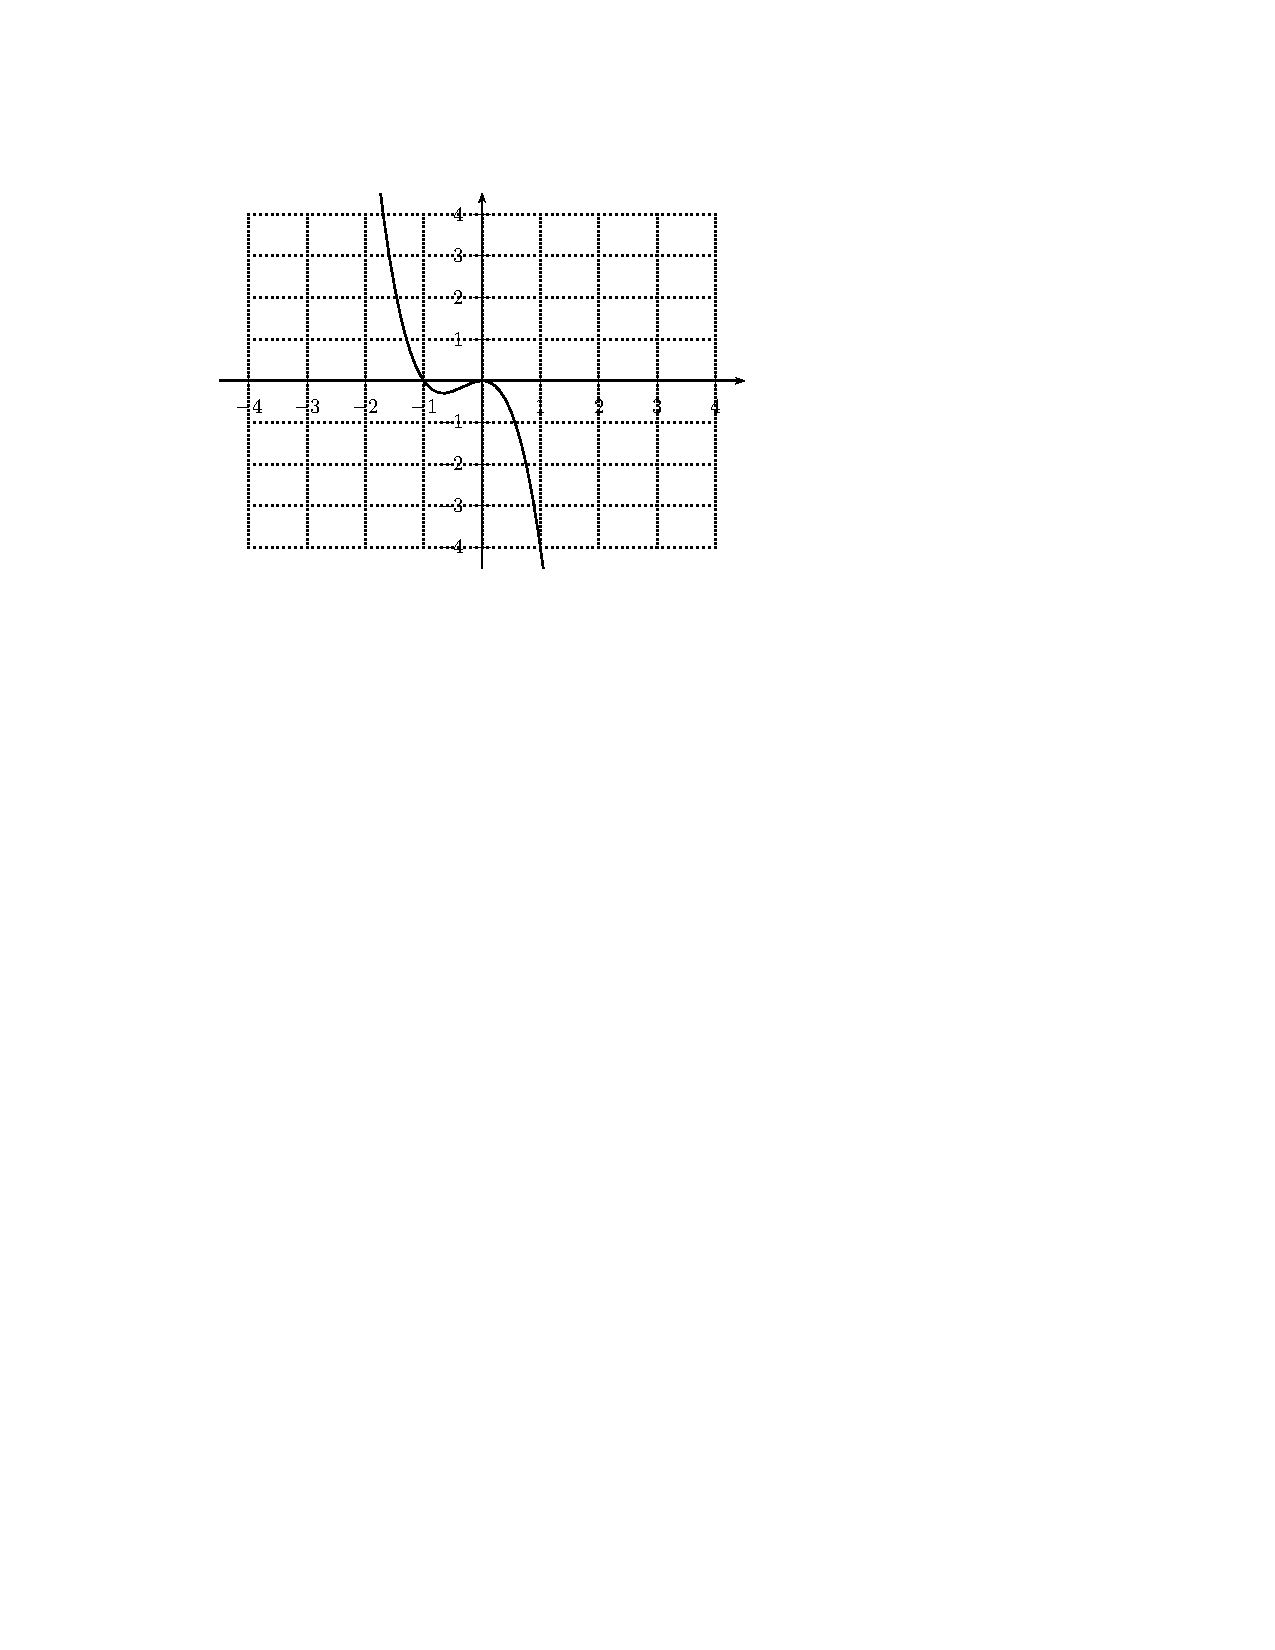
\includegraphics[width=3.5in]{graph}
\end{minipage}\hfill
\begin{minipage}[t]{\linewidth-3.5in-30pt}\vskip\baselineskip\kern0pt
\noindent\makebox[\linewidth][c]{\textbf{Work Area}}
\begin{itemize}
\item The end-behavior is like $y=-x^3$
\item $x$-int: $x=0$ (even); $ x=-1 $ (odd)
\item $y$-int: $y=0$ (passes through origin)
\end{itemize}
\end{minipage}
\end{solution}
\begin{workarea}{\sameVspace}%
\begin{minipage}[t]{3.5in}\kern0pt
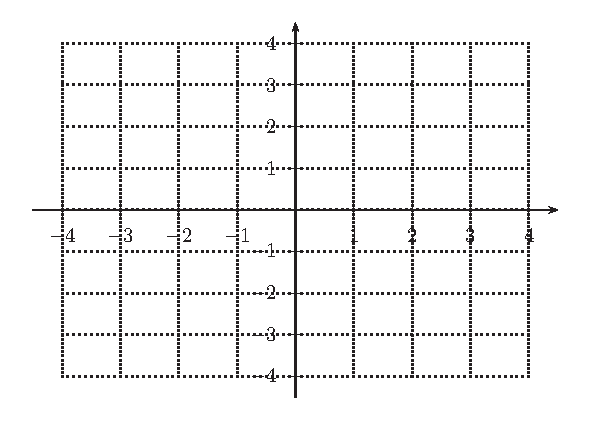
\includegraphics[width=3.5in]{coorplane}
\end{minipage}\hfill
\begin{minipage}[t]{\linewidth-3.5in-30pt}\kern0pt
\makebox[\linewidth][c]{\textbf{Work Area}}
\end{minipage}
\end{workarea}
\end{problem}

\begin{eqComments}[Comments:]
Finally, we have the above problem. It uses the \texttt{workarea}
environment. Previously, \texttt{workarea} appeared with the \texttt{nosolutions}
option. Now it appears with the \texttt{vspacewithsolns} option as well.
On the actual test, I used \textsf{PSTricks} for the graphics, for this
demo file, I replace the \textsf{pstricks} code this a figure depicting what the
\textsf{pstricks} produced, that way users of pdflatex can compile this
file! \texttt{:-)}
\end{eqComments}

\newpage

\begin{eqComments}%
On this page, we more clearly demonstrate the new feature of preserving
the vertical space even when the \texttt{answerkey} option is used. In the
preamble, we have \cs{vspacewithkeyOn}.
\end{eqComments}


\resetSolnAfterToDefault
% try changing \vspacewithkeyOn to \vspacewithkeyOff and recompile,
% the 4 inches of vertical space are not preserved when you compile
% with the answerkey option.
\vspacewithkeyOn

\begin{problem}[10]
Solve the equation $2x^2 - 5x + 10 = 0 $ using the quadratic formula.
\begin{solution}[4in]
Applying the quadratic formula with $a=2$, $ b = -5 $, and $ c = 10 $,
\begin{alignat*}{2}
    x & = \frac{-b \pm \sqrt{b^2 -4ac}}{2a} \qt{The Quad.\ Formula}\\&
        = \frac{5 \pm \sqrt{25 -4(2)(10)}}{2(2)} \qt{substitute}\\&
        = \frac{5 \pm \sqrt{25 -80}}{4} \qt{arithmetic}\\&
        = \frac{5 \pm \sqrt{-45}}{4} \qt{ditto}\\&
        = \frac{5 \pm 3\sqrt{5}\,\imath}{4} \qt{simplify}
\end{alignat*}
The solution is $\boxed{x=\frac{5 \pm 3\sqrt{5}\,\imath}{4}}$
\end{solution}
\end{problem}

\begin{problem}[5]
Write the equation, in standard form, for the circle with center at
$C(1,-3)$ and radius of $2$
\begin{solution}[1in]
We have $(x-1)^2 + (y+2)^2 = 4 $. Expanding and combining the equation, we
have\dots \[\boxed{x^2+y^2-2x+4y+1=0}\]
\end{solution}
\end{problem}

\begin{eqComments}[Comments:]
The \texttt{solution} environments in the above problems declared 4 inches
and 1 inch of vertical space, respectively. With \cs{vspacewithkeyOn} we
should have about 4 inches (resp., 1 inch) of vertical space even with the
\texttt{answerkey} option. Try compiling the file with
\cs{vspacewithkeyOff}.
\end{eqComments}

\end{theseproblems}

\end{exam}

\end{document}
